% Ppopy Phase 2 Submission B
% Reconstructed from the latest Revised PDF, with the title spelling Ppopy.
% This file contains the complete document; IEEEtran.cls is included alongside it.
\documentclass[conference,letterpaper]{IEEEtran}
\usepackage[T1]{fontenc}
\usepackage{courier}
\usepackage{amsmath,amssymb}
\usepackage{booktabs,array,tabularx,cite,url,listings,xcolor,tikz}
\usepackage[hidelinks]{hyperref}
\urlstyle{same}
\hypersetup{pdftitle={Ppopy: Proactive Skincare Decision Support with a Smart Mirror},pdfauthor={Doyeong Koo; Takgeon Kang; Geonil Won}}
\lstset{basicstyle=\ttfamily\footnotesize,breaklines=true,columns=fullflexible,keepspaces=true,showstringspaces=false,frame=single,rulecolor=\color{gray},aboveskip=5pt,belowskip=5pt,xleftmargin=2pt,xrightmargin=2pt}
\title{Ppopy: Proactive Skincare Decision Support with a Smart Mirror}
\author{\IEEEauthorblockN{Doyeong Koo, Takgeon Kang, Geonil Won}\IEEEauthorblockA{Hanyang University\\Team CosMate -- CSE406 Software Engineering}}
\begin{document}
\maketitle
\pagestyle{plain}
\thispagestyle{plain}
\begin{abstract}
Team CosMate proposes ppopy to help users decide what to maintain, adjust or check before their skincare routine. The system compares confirmed product information, planned routines and reported use with a knowledge base (KB), and requests only information that can change a decision. For proactive guidance, it estimates the next routine start from user-confirmed use times, selects any needed guidance and displays it on a previously authorized smart mirror before that start. The mirror provides an overview at the washbasin or vanity; users answer questions and approve routine changes in the app. The prototype combines context-sensitive decisions with advance delivery on one home display.
\end{abstract}
\begin{IEEEkeywords}skincare decision support, knowledge base, proactive guidance, smart mirror\end{IEEEkeywords}
\section*{Team Responsibilities}
{\centering\footnotesize
\renewcommand{\arraystretch}{1.12}\setlength{\tabcolsep}{3pt}
\begin{tabularx}{\columnwidth}{@{}>{\hsize=.70\hsize\raggedright\arraybackslash}X>{\hsize=1.30\hsize\raggedright\arraybackslash}X@{}}\toprule
\textbf{Member(s)} & \textbf{Responsibilities}\\\midrule
All members & Data collection, user needs review, development planning, integration testing and project decisions\\
Doyeong Koo & App and backend development, KB construction and system integration\\
Takgeon Kang & Agent workflow, contextual follow-up questions and guidance selection\\
Geonil Won & Smart mirror hardware, display client and app--device integration\\
\bottomrule
\end{tabularx}
}

\section{Introduction}

\subsection{Problem and Objective}

The project addresses a practical need: deciding how to carry out a skincare routine and what to check before starting it. A product list alone does not explain which part of a user's planned routine needs attention. ppopy combines confirmed products, actual-use reports, user goals and KB criteria to select relevant guidance. A mirror at the washbasin or vanity makes that guidance available while the user prepares for the routine.

\subsection{User Workflow and Example}

Users register products by name, photo or screenshot, confirm the product and variant, and record their plan and actual use. They set a goal such as ``show what I need to check before starting.'' The system reviews the plan and context, asks decision-changing questions in the app, and updates its findings after answers.

For example, three confirmed evening starts at 20:56, 21:00 and 21:04 produce an estimated start of 21:00. At 20:50, the system reviews the upcoming routine. It may select an adjustment, request a missing fact, or find no need for new guidance. With valid prior display approval, needed guidance appears on the mirror before 21:00. The estimated time determines when to review; the KB and user context determine what to do.

\subsection{Related Software}

SkinSort's routine creator supports routine organization \cite{ref1}; INKEEDecoder explains ingredient lists \cite{ref2}. These functions inform ppopy's product and routine presentation. The proposed workflow connects use-context comparison, decision-dependent questions and advance guidance on a home display.

\subsection{Prototype Scope and Current Status}

Development work includes product-input components, a local React/Python KB review, follow-up questions and account-separated JSON records \cite{ref3}. The course prototype will integrate these components with history-based timing, automatic delivery, real account authentication, cloud storage and one output-only mirror. Questions, settings and plan approval remain in the app. Time and weather form the mirror's default screen; broader appliance orchestration is future work. The timing estimate concerns the next routine start, not future skin condition.

\section{Requirements}

\subsection{Functional Requirements}

\subsubsection*{R1. Sign-in and consent}

Require sign-in and appropriate consent for personal routine records; restrict each record to its owner.

\subsubsection*{R2. Product registration and ingredients}

Confirm products and variants from names, photos or screenshots. Verify ingredient sources, product versions and standard-name matches before using them as facts.

\subsubsection*{R3. Plans, actual use and user intent}

Keep confirmed plans separate from actual-use reports. Allow edits to the time, products, use details and reported discomfort, and let users set guidance goals and preferences.

\subsubsection*{R4. Contextual KB review}

Review current and planned routines against applicable KB criteria and exceptions. Distinguish confirmed facts from unknown or conflicting information.

\subsubsection*{R5. Decision-dependent questions}

Ask only for unknown information that can change a decision. Update related findings after answers; preserve skipped or declined answers as unknown without repeating a question in unchanged context.

\subsubsection*{R6. Decision and guidance selection}

Select maintain, adjust, check or defer with linked reasons and evidence. Preserve the decision when no new user-facing intervention is needed. A suggestion changes the confirmed plan only after explicit app acceptance.

\subsubsection*{R7. Separate records and outcomes}

Store plans, suggestions, actual-use reports, time estimates, decisions and delivery/display outcomes separately, with their revisions and origins.

\subsubsection*{R8. Mirror pairing and display approval}

Pair one output-only mirror. Configure its room, timezone, default screen, allowed display periods and approval expiry in the app.

\subsubsection*{R9. Next-time estimation and proactive guidance}

Estimate the next routine start from valid actual-use times and review the latest context beforehand. Display needed, current guidance before that start within prior approval; prevent duplicates and invalidate outdated decisions or commands.

\subsubsection*{R10. Account and display controls}

Provide logout, consent/display-approval withdrawal and account deletion. End personal access and expire displayed content when authority ends; distinguish a deletion request from completed cleanup.

\subsection{Quality Requirements}

\subsubsection*{Q1. Personal information protection}

Protect transmission and storage. Authorize personal mirror content by account, paired device and valid display approval, without inferring who is viewing the mirror.

\subsubsection*{Q2. Reliable execution and accessibility}

Discard stale guidance, prevent duplicate interventions and record only acknowledged delivery stages. Show errors clearly and support readable Korean controls, enlarged text and VoiceOver.

\subsubsection*{Q3. Traceability and verification}

Link estimates and decisions to inputs, parameters, KB sources and execution outcomes. Map R1--R10/Q1--Q3 to reproducible tests and distinguish planned tests from executed evidence.
\section{Development Environment}

\subsection{Platforms, Languages and Versions}

React and TypeScript provide the app's editable routines, questions and guidance views. Typed request/response structures help distinguish missing information from confirmed answers \cite{ref4}. Capacitor packages the interface for iOS and connects the product-image bridge \cite{ref5}; Vite supports development and builds. Python implements source verification, explicit KB rules and time estimation without a trained prediction model. The cloud target uses API Gateway/Lambda for the service and Aurora PostgreSQL for account-linked storage.

Table I separates the recorded development environment from deployment targets. The local KB service uses Python 3.9.6 and account-separated JSON storage. Compatibility with Python 3.9 and the Lambda 3.12 target will be checked using the same decision and timing fixtures. Standard-library IANA timezone support provides local/UTC conversion \cite{ref6}.

The mirror target is a full-screen React view on a Raspberry Pi connected to a monitor over HDMI \cite{ref7}. Pi 5 2GB is the initial sizing and cost reference. Power, microSD storage, cooling, cabling and mounting are included in the procurement scope; final compatibility depends on the selected board.

\begin{table}[!t]
\caption{Development Environment and Deployment Targets}\label{tab:env}
\centering\footnotesize
\renewcommand{\arraystretch}{1.12}\setlength{\tabcolsep}{3pt}
\begin{tabularx}{\columnwidth}{@{}>{\raggedright\arraybackslash}X>{\raggedright\arraybackslash}X@{}}\toprule
\textbf{Item} & \textbf{Recorded environment or target}\\\midrule
Development computer & MacBook Pro M4 Pro; 12 CPU cores; 24 GB RAM\\
OS / native tools & macOS 26.3.1 / Xcode 26.6\\
Python / Node.js & KB development: 3.9.6; system: 3.14.7 / Node.js 24.13.0\\
Interface packages & React 19.2.8; TypeScript 5.9.3; Vite 7.3.6; Capacitor 8.5.1\\
Test packages & Vitest 3.2.7; Playwright 1.62.1; pytest 8.4.2\\
Cloud target & Lambda Python 3.12; Aurora PostgreSQL\\
Mirror target & Raspberry Pi, full-screen browser, Wi-Fi/HDMI; model and OS/browser versions to be selected\\
\bottomrule
\end{tabularx}
\end{table}

\subsection{Software and Integration Scope}

The product-input pipeline uses an LLM to extract visible identity clues and obtain source-linked ingredient drafts when catalog data are missing. Product confirmation, source checks and dictionary matching determine which facts are usable. KB decisions use explicit Python conditions. The timing component uses statistics over user-confirmed actual-use records, while a periodic service check and mirror polling support automatic delivery. Integration with real account authentication and cloud storage is planned alongside the mirror functions described in Section I-D.

\subsection{Cost Estimate}

Table II covers one development month, one annual Apple Developer payment and one mirror. Subscription amounts are project-reported charges; hardware amounts are reference estimates. The listed controller, power supply and cooler are priced separately \cite{ref8}, \cite{ref9}, \cite{ref10}. The recorded board listing was sold out, so final availability and model selection remain procurement tasks.

The AWS model assumes a Seoul Aurora service averaging 0.5 ACU for 720 hours, 10 GB storage and 100,000 monthly API requests. One service check and one mirror poll per minute imply approximately 86,400 checks/requests per 30 days before app traffic. The estimate assumes continuous availability because frequent database access can limit auto-pause. The modeled monthly charge is approximately USD 82.01, budgeted as USD 83 at KRW 1,400/USD, or KRW 116,200 \cite{ref11}.

The API allowance assumes 100 image registrations, a 95\% usable catalog-match rate and two web searches per miss. The modeled cost is about KRW 5.70 per registration, rounded to KRW 600 in total \cite{ref12}. KB review and time estimation require no paid-model calls. These rates and the match rate are budget assumptions rather than measured operating costs.

The priced subtotal is KRW 667,484. A complete total also requires quotes for the pending items. The cooler reference includes VAT; other components retain their reported/listed amounts. AWS/API taxes, card or exchange charges and additional delivery are outside the subtotal. Excluding the optional epoxy reduces it by KRW 5,900.

\begin{table}[!t]
\caption{Project Budget: Priced Items and Pending Costs}\label{tab:cost}
\centering\footnotesize
\renewcommand{\arraystretch}{1.12}\setlength{\tabcolsep}{3pt}
\begin{tabularx}{\columnwidth}{@{}>{\raggedright\arraybackslash}X>{\raggedright\arraybackslash}X@{}}\toprule
\textbf{Item / quantity or period} & \textbf{KRW}\\\midrule
ChatGPT Pro 100, 1 month & 144,545\\
Apple Developer, 1 year & 129,000\\
AWS, 1 month, always available & 116,200\\
Product-input API, 100 registrations & 600\\
Existing development computer / iPhone & 0\\
27-inch monitor, 1 & 95,000\\
3 mm acrylic sheet, 1 & 10,740\\
Reflective film, 1 & 6,200\\
Spray bottle, 1 & 2,220\\
Rubber squeegee, 1 & 1,980\\
VHB double-sided tape, 3 m & 7,800\\
Epoxy adhesive, 1 (optional, included) & 5,900\\
Estimated material delivery & 8,500\\
Subtotal before controller items & 528,685\\
Raspberry Pi 5 2GB reference & 114,400\\
5V/5A USB-C power supply reference & 17,000\\
Pi 5 Active Cooler reference & 7,399\\
Priced-items subtotal & 667,484\\
microSD 32GB; micro-HDMI/HDMI cable & Pending\\
Case/mounting/frame; additional delivery & Pending\\
\bottomrule
\end{tabularx}
\end{table}

\section{Specifications}

\subsection{Processing Flow}

Figure 1 summarizes the proposed loop. The app sends confirmed inputs as JSON. Python returns findings, relevant questions, selected guidance and evidence references. A personal mirror message contains only the selected display fields, command ID, revisions and deadlines. Manual review remains available; prior approval also permits automatic execution before the expected routine start.

\begin{figure}[!t]
\centering
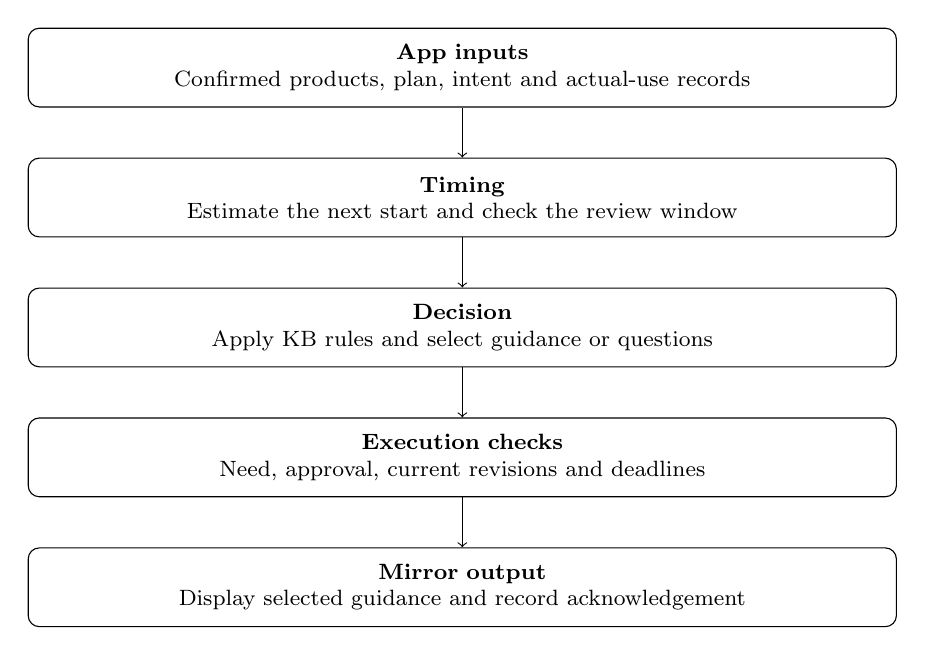
\begin{tikzpicture}[every node/.style={align=center,font=\footnotesize},box/.style={draw,rounded corners,text width=.89\columnwidth,minimum height=1cm}]
\node[box] (i) at (0,0) {\textbf{App inputs}\\Confirmed products, plan, intent and actual-use records};
\node[box] (t) at (0,-1.65) {\textbf{Timing}\\Estimate the next start and check the review window};
\node[box] (d) at (0,-3.3) {\textbf{Decision}\\Apply KB rules and select guidance or questions};
\node[box] (c) at (0,-4.95) {\textbf{Execution checks}\\Need, approval, current revisions and deadlines};
\node[box] (o) at (0,-6.6) {\textbf{Mirror output}\\Display selected guidance and record acknowledgement};
\draw[->] (i)--(t);\draw[->] (t)--(d);\draw[->] (d)--(c);\draw[->] (c)--(o);
\end{tikzpicture}
\caption{Proposed processing loop. App answers and later actual-use reports update the inputs. Without needed, authorized guidance, the mirror keeps its default screen.}\label{fig:flow}
\end{figure}

\subsection{Decisions and an Illustrative Example}

The KB review produces a result for each relevant rule. Maintain means the confirmed practice meets the rule; adjust identifies a supported change; check requests an answer that could change the result; and defer leaves an issue unresolved. A rule that does not apply is excluded. Table III shows the main branches.

The display choice is separate from the review result. No intervention means no new user-facing guidance is needed; it does not resolve a deferred issue. Repeated guidance is suppressed according to user intent and notice history. A preference for fewer messages alone must not suppress a currently needed, source-supported exception. All displayed content still passes approval, freshness and duplicate checks.

For the 21:00 example in Section I-B, consider the development KB's lukewarm face-washing entry, B-C01, linked to the American Academy of Dermatology source \cite{ref13}, \cite{ref3}. Assume an applicable facial-cleansing plan, no conflicting individual/product instruction and no reported discomfort. Table IV illustrates how the same review time can lead to different actions. A suggested change becomes part of the plan only after acceptance in the app.

\begin{table}[!t]
\caption{KB Review Outcomes}\label{tab:outcomes}
\centering\footnotesize
\renewcommand{\arraystretch}{1.12}\setlength{\tabcolsep}{3pt}
\begin{tabularx}{\columnwidth}{@{}>{\raggedright\arraybackslash}X>{\raggedright\arraybackslash}X@{}}\toprule
\textbf{Confirmed context or uncertainty} & \textbf{Review outcome}\\\midrule
Rule does not apply to this routine & Exclude the rule; no guidance from it.\\
An unknown answer could change the result & Check if an answer can be requested; otherwise defer.\\
Instructions conflict, or required evidence is missing & Defer; request useful clarification without assuming a conclusion.\\
Discomfort is reported & Use only a source-supported exception, classified as adjust or check; otherwise defer.\\
Confirmed practice differs from an applicable KB criterion & Adjust, with a specific reason and evidence.\\
Confirmed practice meets the criterion & Maintain; a reminder is optional.\\
\bottomrule
\end{tabularx}
\end{table}

\begin{table}[!t]
\caption{Different Decisions at the Same Review Time}\label{tab:example}
\centering\footnotesize
\renewcommand{\arraystretch}{1.12}\setlength{\tabcolsep}{3pt}
\begin{tabularx}{\columnwidth}{@{}>{\raggedright\arraybackslash}X>{\raggedright\arraybackslash}X@{}}\toprule
\textbf{Input for the upcoming routine} & \textbf{Decision and guidance}\\\midrule
Water is confirmed as hot & Adjust: show the KB-supported lukewarm-water guidance before the routine.\\
Water temperature is unknown & Check: request the missing fact in the app; do not infer a difference.\\
Plan follows the rule; the same reminder adds no value & Maintain the review result; select no new intervention.\\
\bottomrule
\end{tabularx}
\end{table}

\subsection{Next-Start Estimation and Timing Parameters}

The estimator treats user-confirmed AM and PM routines separately. It uses the latest seven valid actual-use reports from the preceding 14 days, taking at most the latest report per local routine date/session. A PM routine date begins at local noon, allowing an after-midnight report to belong to the preceding evening. A cycle is identified by account, local routine date and AM/PM session.

A valid report belongs to the account/session, explicitly records actual use, has a parseable UTC start and the current configured IANA timezone, and is neither deleted, future-dated nor duplicated. System estimates, app/display events and synthetic fixtures do not enter operational estimation.

Convert valid starts to local clock minutes $m\in[0,1440)$. The circular distance is \begin{equation}
d(a,b)=\min\bigl(|a-b|,1440-|a-b|\bigr).
\end{equation}

Choose an observed minute $m^*$ that minimizes the sum of distances to the observations, breaking ties by the most recently reported candidate. This keeps 23:55 and 00:05 close together. Use this history estimate only with at least three distinct routine dates and a median circular deviation of at most 60 minutes. Otherwise, use an explicitly configured user time, or return no timing basis.

The next start is the nearest future, uncompleted local occurrence for that session, converted to UTC. An ambiguous or nonexistent daylight-saving occurrence is skipped and requires app confirmation. Timezone, plan or history corrections invalidate the old estimate and pending command. The method label distinguishes history\_estimate from the user\_schedule fallback. Products are taken from the confirmed plan.

\begin{lstlisting}
records = valid_reports(last_days=14, limit=7)
if distinct_dates(records) >= 3:
  m = circular_sample_median(records)
  if median_distance(records, m) <= 60:
    return (next_future_cycle(m),
            "history_estimate", record_ids)
if explicit_user_time_exists():
  return (next_future_cycle(user_time),
          "user_schedule")
return none, "no_time_basis"
\end{lstlisting}

Table V gives the initial design parameters. The first-display deadline determines whether an intervention was proactive. A separate retention expiry limits how long guidance that appeared in time may remain visible. These settings are design choices to be evaluated during integration.

\begin{table}[!t]
\caption{Initial Timing and Delivery Parameters}\label{tab:timing}
\centering\footnotesize
\renewcommand{\arraystretch}{1.12}\setlength{\tabcolsep}{3pt}
\begin{tabularx}{\columnwidth}{@{}>{\raggedright\arraybackslash}X>{\raggedright\arraybackslash}X@{}}\toprule
\textbf{Parameter} & \textbf{Initial value}\\\midrule
Lookback / maximum reports & 14 days / 7 per AM/PM session\\
Minimum history / dispersion & 3 routine dates / median deviation $\leq$60 min\\
Review lead / service check & 10 min / 60 s\\
First-display deadline & Strictly before estimated start T\\
Fixed retention expiry & Earliest of T + 5 min, request time +15 min, grant end and window end\\
Device poll / display lease & 60 s / at most 90 s per renewal, bounded by retention expiry\\
Command transmissions & At most 2 total with the same ID, both before T\\
\bottomrule
\end{tabularx}
\end{table}

\subsection{Requirement-Level Processing and Verification}

The following specifications describe the target behavior under the environment in Section III. Each verification paragraph is a planned check; the integrated proactive path has not yet produced acceptance results.

\subsubsection*{R1. Sign-in and consent}

The Capacitor app sends a login result to the Python API. Before returning a record, the server validates the session, record ownership and consent required for the operation. React opens the workspace after authorization. Local development sessions currently use synthetic accounts.

\begin{lstlisting}
account = verify_session(login_result)
if not account: return login_required
if not has_consent(account):
  return consent_required
return records_owned_by(account)
\end{lstlisting}



\textit{Verification plan:} Test valid/expired sessions, missing consent and a second account. Only the authorized owner may read or edit personal records.

\subsubsection*{R2. Product registration and ingredients}

React accepts a name, camera photo or uploaded screenshot. The user crops/confirms the product area; the Capacitor bridge sends it for extraction of visible brand, name and variant. These clues search the catalog, and the user confirms the result. Unclear images fall back to name search.

Python reads catalog ingredients first. If unavailable, source-linked LLM search returns a draft with product identity, raw ingredients and URL. The service verifies the product/version, preserves the original text and matches tokens against a standard-name/alias dictionary. Unresolved identities or names remain unconfirmed.

\begin{lstlisting}
clues = read_name_or_image(app_input)
matches = search_catalog(clues)
product = app_confirm_product(matches)
raw = catalog_ingredients(product)
if raw is missing:
  raw = source_linked_lookup(product)
if not matches_product_version(raw, product):
  return check_required
return verify_text_and_names(raw)
\end{lstlisting}



\textit{Verification plan:} Test all three input methods, similar variants and unresolved ingredient terms. Preserve the selected product and sources; unresolved evidence must not become a confirmed KB fact.

\subsubsection*{R3. Plans, actual use and user intent}

React provides separate plan and actual-use editors. A report contains user-declared start time, timezone, AM/PM session, products, order, amount, frequency, use/combined-use method, discomfort and revision. Intent specifies guidance goals and repeat preferences. Suggestions do not populate actual-use records. Corrections increment the input revision and invalidate pending guidance.

\begin{lstlisting}
if entry.kind == "actual_use":
  require_confirmed_time_and_timezone(entry)
  save_report(entry, origin="user_report")
else:
  save_plan_or_preference(entry)
on_edit:
  increment_revision()
  invalidate_pending_guidance()
\end{lstlisting}



\textit{Verification plan:} Add/edit/reorder products and correct a use time. Reopening preserves the plan/report distinction; changed inputs invalidate old decisions. App/display events do not increase the actual-use count.

\subsubsection*{R4. Contextual KB review}

Each KB rule contains applicability conditions, required observations, exceptions, actions and source IDs. Python reviews the upcoming confirmed plan and latest reported context. A known inapplicable rule is excluded; unknown applicability leads to a relevant question or defer. Product facts come from evidence, not user guesses.

Applicable individual care directions and product instructions take priority over general KB guidance. Unclear scope or conflicting instructions cause defer and clarification for that item. Reported discomfort prevents an unqualified maintain result: only a source-supported exception can supply guidance. Independent items can still be reviewed. Every branch retains its inputs, sources and reason.

\begin{lstlisting}
for rule in KB:
  scope = applies_to(rule, plan, context)
  if scope is False:
    result = excluded
  elif scope is unknown:
    result = check_or_defer(rule)
  elif directions_conflict_or_unclear(rule):
    result = defer_with_reason(rule)
  elif reported_discomfort(rule):
    result = supported_exception_or_defer(rule)
  elif missing_required_fact(rule):
    result = check_or_defer(rule)
  else:
    result = compare_confirmed_facts(rule)
  save_result(result, inputs, sources, reason)
\end{lstlisting}



\textit{Verification plan:} Test applicable, excluded, unknown and conflicting cases. Missing values cannot establish a difference; discomfort cannot produce unqualified reassurance. Trace data must exist for early-exit cases as well as ordinary comparisons.

\subsubsection*{R5. Decision-dependent questions}

For an applicable rule, Python checks whether different permitted answers could change the result or next action. Only those unknown observations become questions. Evidence-only fields trigger product lookup. A question key includes product, context and relevant input revision. Skipped/declined answers remain unknown and suppress that question until context changes or the user reopens it.

\begin{lstlisting}
for field in unresolved_fields(rule):
  if not answer_changes_decision(field):
    continue
  if evidence_only(field):
    request_product_evidence(field)
  elif not handled_in_same_context(field):
    add_question(field, choices,
                 reason, rule.id)
on_answer:
  save_answer_and_revision()
  invalidate_pending_guidance()
  return review_latest_input()
\end{lstlisting}



\textit{Verification plan:} Test relevant/irrelevant unknowns, answers, refusal and skipping. Answering updates related findings; declined questions do not repeat in unchanged context.

\subsubsection*{R6. Decision and guidance selection}

Apply Table III after R4/R5. Preserve each review result independently of the display choice. Select guidance using user intent, novelty and notice history. No intervention can coexist with a deferred issue or a maintained routine. Needed source-supported exception guidance remains eligible even when the user prefers fewer messages; permission, freshness and duplicate checks still apply.

Each result links facts, plan revision, KB/source IDs and its reason. React shows the proposal; only explicit acceptance commits a plan edit.

\begin{lstlisting}
result = apply_decision_table(findings)
content = actionable_content(result, questions)
notify = (content_exists(content)
          and new_or_needed(content, intent,
                            history))
if needed_supported_exception(content):
  notify = True
save_review(result, inputs, sources, reason)
save_display_choice(content if notify else none)
on_app_acceptance: commit_plan_edit()
\end{lstlisting}



\textit{Verification plan:} Test a needed adjustment, no added value, missing facts, conflicts and a rejected suggestion. Suppression preserves the underlying result and evidence. Without acceptance, the confirmed plan and actual-use records stay unchanged.

\subsubsection*{R7. Separate records and outcomes}

The service stores distinct plan, actual-use, review, timing-estimate, intervention and delivery-event objects. Estimates include method, report IDs and parameter version; events include command/device IDs and timestamps. Origins distinguish user reports, system estimates and synthetic fixtures. A later report links to a new review without overwriting the earlier decision. A suggestion, accepted edit, displayed view and reported use are separate outcomes.

Account-separated JSON is the development store; PostgreSQL is the cloud target. Versioned records support traceability and invalidation.

\begin{lstlisting}
save_plan_or_report(record, revision, origin)
save_review_and_display_choice(result, choice)
save_estimate(method, report_ids, parameters)
append_event(command_id, stage, device_id, time)
on_later_report: link_new_review_to_previous()
\end{lstlisting}



\textit{Verification plan:} Reopen and trace estimates to reports and decisions to input/KB versions. A display event must not create either an actual-use report or an accepted plan edit.

\subsubsection*{R8. Mirror pairing and display approval}

The app pairs one mirror and records its room label, IANA timezone, allowed display windows and finite approval expiry. A display grant is this account's permission to show selected personal guidance on that device. The mirror accepts no user input; answers, plan acceptance and settings remain in the app. Its default view shows time and weather.

The mirror polls every 60 seconds. Each successful response checks the device, grant, window and command revisions. The server issues a display lease: a temporary permission to keep the current content visible. Its end is the earlier of server time plus 90 seconds and the fixed retention expiry in Table V. Failed refreshes cannot extend it; local expiry clears the screen even offline.

A command ID produces only one initial display. An authorized reply can renew its still-active view without mounting it again. A cleared view is not restarted under the same ID. If an acknowledgement was lost, the device can resend its saved acknowledgement with the original first-display time. Ordinary polling, lease renewal and saved acknowledgement transmission do not count as command delivery attempts.

\begin{lstlisting}
on_boot: show_default_view()
every_60_seconds: poll_server()
on_poll_reply(r):
  if r.denied_or_stale:
    clear_personal_view(); return
  if not valid_reply(r): return
  if has_rendered(r.id):
    if active_id == r.id: renew_to(r.lease_end)
    resend_saved_render_ack(r.id)
    return
  send_received_ack(r.id, utc_now())
  t = render_first_if_valid(r)
  if t is none: return
  remember_render(r.id, t, r.lease_end)
  send_render_ack(r.id, t)
on_local_expiry: show_default_view()
\end{lstlisting}

The initial view checks both deadlines before mounting: the time must be before T and within its issued lease. Its acknowledgement reports the mount time, not command receipt. Device/server timestamps use UTC; integration checks their clock agreement, while scenario tests use controlled clocks.

\textit{Verification plan:} Test pairing, settings, weather outage, permission expiry/revocation, duplicate IDs, acknowledgement loss and offline expiry. Renewal preserves an active view without another display event. Online revocation clears at the next poll, within 60 seconds; loss of connectivity cannot extend the last lease beyond 90 seconds or an earlier expiry.

\subsubsection*{R9. Next-time estimation and proactive guidance}

A Python development loop or scheduled service invocation checks once per minute. It reads current records, invalidates commands whose input/plan/KB/intent/grant revision changed, and cancels a cycle's pending guidance when the user reports it complete. For the next eligible AM/PM cycle, review runs only in [T - 10 min,T).

R4--R6 determine the review result and display choice. No timing basis, no needed guidance or no valid display grant produces no personal command. An atomic claim rechecks authority and revisions, ensuring one logical command ID per decision/cycle even when checks overlap. All subsequent delivery and renewal operations retain that ID and its original deadlines.

\begin{lstlisting}
every_60_seconds:
  state = read_latest_state()
  cancel_stale_or_completed(state)
  estimate = estimate_next_start(state)
  save_estimate_and_basis(estimate)
  if estimate is none: continue
  T = estimate.start
  if not (T-10min <= now < T): continue
  result, content = review_and_select(state)
  if content is none: continue
  if not valid_display_authority(state):
    continue
  c = claim_once(content, cycle, revisions)
  if c is none: continue
  c.first_deadline = T
  c.keep_until = min(T+5min, now+15min,
                     grant_end, window_end)
  queue_command(c)
\end{lstlisting}

The first display must occur strictly before T. A view displayed in time can remain until the earlier of its current lease end and keep\_until. Initial transmission and any retransmission are limited to two total attempts, both before T. Retries and renewals do not reset either deadline. A mirror's ordinary no-command poll is not a delivery attempt.

Queued, sent, device-received and view-rendered stages are recorded separately. Both acknowledgements must come from the authenticated device assigned to the command. A valid view acknowledgement supplies first\_rendered\_at; its server arrival time is recorded separately.

The reported first-display time must lie within an issued lease, precede T and be no later than acknowledgement arrival.

A delayed acknowledgement may confirm an eligible earlier display while the command is current and before its fixed retention expiry. It cannot authorize a late first display or extend a lease. An expired short lease does not erase evidence of a display that occurred within it.

\begin{lstlisting}
on_command_delivery(c):
  if not current_authorized(c): return none
  if now >= c.first_deadline: return none
  if c.attempts >= 2: return none
  c.attempts += 1
  return transmit_same_id(c)
on_received_ack(id, t):
  if not valid_ack_origin(id): return
  save_received_once(id, t, utc_now())
on_view_ack(id, t):
  if not valid_ack_origin(id): return
  if current_before_retention_expiry(id):
    if valid_first_render_time(id, t):
      save_rendered_once(id, t, utc_now())
      return
  reject_ack(id)
on_missing_ack: keep_delivery_unconfirmed()
\end{lstlisting}



\textit{Verification plan:} Test pre-start guidance, no intervention at the same time, changed/sparse history, edited inputs, duplicate checks, expired authority and connection failure. A first display at or after T fails proactive acceptance. A valid delayed acknowledgement confirms its original display time; missing/invalid acknowledgement remains unconfirmed.

\subsubsection*{R10. Account and display controls}

React submits distinct logout, consent withdrawal, grant revocation and account-deletion requests. Python invalidates affected sessions/grants and pending commands before returning status. New personal reads and lease renewals stop at the server immediately. The mirror returns to its default view on the next check or earlier local expiry, within R8's bounds. Cleanup progresses through requested, in-progress and completed states.

\begin{lstlisting}
on_logout_withdrawal_or_grant_end:
  revoke_authority()
  cancel_pending_commands()
  block_personal_reads_and_renewals()
  app.clear_personal_state()
on_device_check_or_expiry: show_default_view()
on_account_delete: request_cleanup()
show_cleanup_state_after_confirmation()
\end{lstlisting}



\textit{Verification plan:} Test each control, including an already displayed command. Revocation blocks server access immediately; the device clears within its check/lease limit. A deletion request is not shown as completed cleanup.

\subsubsection*{Q1. Personal information protection}

Cloud traffic uses HTTPS and protected account-linked storage. Every personal response validates the account, paired device, display scope and unexpired grant. Device messages and logs omit full questionnaire answers and credentials. Room labels are configuration only. Approval authorizes a display device and does not identify a viewer; the app explains shared-screen exposure and provides revocation.

\begin{lstlisting}
authorize(account, device, scope, grant_expiry)
if unauthorized: return default_view_only
return minimum_approved_display_fields()
log(command_id, stage, reason_code)
\end{lstlisting}



\textit{Verification plan:} Test cross-account/device requests, revoked grants and sampled responses/logs. Unauthorized requests reveal no personal guidance.

\subsubsection*{Q2. Reliable execution and accessibility}

Revision checks reject stale findings and commands. Request IDs prevent duplicate saves; an uncertain save is read back before retry. Decision/cycle keys and command IDs prevent duplicate interventions and displays. Unacknowledged delivery stays unknown. React shows progress/errors, and the mirror enforces local expiry.

\begin{lstlisting}
if reply.revision != current_revision:
  discard(reply)
save_once(request_id)
claim_once(decision_cycle_key)
retry_same_id_before_first_deadline()
if no_render_ack: status = "unconfirmed"
expire_personal_content_locally()
\end{lstlisting}



\textit{Verification plan:} Test interruption, stale replies, duplicate checks/commands and missing acknowledgements. Target warm catalog-search p95 at most 3 s and KB-review p95 at most 5 s over at least 30 runs each, excluding external lookup. Inspect Korean controls at 320 px width, 200\% text and with iOS VoiceOver. Timing/delivery deadlines are checked separately.

\subsubsection*{Q3. Traceability and verification}

Each test case links to a requirement ID. A trace records input/plan/KB versions, estimate parameters, decision reason, display choice and device-event stages. pytest covers decision, timing and API cases; Vitest covers React updates and expiry; Playwright covers end-to-end app/mirror flows. Git revisions and dependency lockfiles identify the tested build.

\begin{lstlisting}
trace = {inputs, plan_revision, KB_sources,
         timing_method, parameters, decision,
         display_choice, events}
run_pytest(decision_time_and_API_cases)
run_vitest(question_and_expiry_cases)
run_playwright(app_and_mirror_scenarios)
save_result(requirement_id, build_id, trace)
\end{lstlisting}



\textit{Verification plan:} Each of the 13 requirements has a reproducible test or inspection with an expected outcome and recorded result. Synthetic flow checks, real user reports and real-device runs are labeled separately.

\subsection{Proactive Acceptance Scenarios}

Table VI lists planned scenarios using controlled clocks and versioned synthetic histories. They check software branches and delivery behavior. They do not measure real-user prediction accuracy or skin improvement.

\begin{table}[!t]
\caption{Planned Acceptance Scenarios}\label{tab:acceptance}
\centering\footnotesize
\renewcommand{\arraystretch}{1.12}\setlength{\tabcolsep}{3pt}
\begin{tabularx}{\columnwidth}{@{}>{\raggedright\arraybackslash}X>{\raggedright\arraybackslash}X@{}}\toprule
\textbf{Scenario / requirements} & \textbf{Acceptance condition}\\\midrule
V1. Needed guidance; R4--R6, R9 & First display occurs before T and is confirmed by a valid view acknowledgement. A delayed acknowledgement may confirm that earlier display; a late first display fails.\\
V2. No intervention; R6, R9 & No useful new guidance means no command at the same review time. The review result remains stored.\\
V3. Missing information; R4--R6 & Check or defer without inventing facts or repeating declined questions. Suppression does not resolve an issue.\\
V4. Changed/sparse history; R3, R7, R9 & Changed records update the estimate. Fallbacks are labeled; no basis means no schedule.\\
V5. Edits, duplicates, renewal; R3, R7--R9, Q2 & Edits invalidate commands. One command and first display per decision/cycle; renewals preserve the active view.\\
V6. Permission or connection loss; R8--R10, Q1--Q2 & Revocation blocks access and renewal. Local expiry clears the view; failed or unknown delivery remains recorded.\\
\bottomrule
\end{tabularx}
\end{table}

Real-device integration will verify pairing, display acknowledgements, clock agreement and revocation behavior. Timing evaluation can compare each stored estimate with the subsequent user-confirmed start, reporting sample count, coverage, fallback rate and absolute timing error. Controlled scenarios, actual-use records and device runs will remain separate evidence sets.
\begin{thebibliography}{00}
\bibitem{ref1} SkinSort, ``Routine creator.'' [Online]. Available: \url{https://skinsort.com/support/the-routine-creator}. Accessed: Nov. 6, 2026.
\bibitem{ref2} INKEEDecoder, ``About INKEEDecoder.'' [Online]. Available: \url{https://inkeedecoder.com/about}. Accessed: Nov. 6, 2026.
\bibitem{ref3} Team CosMate, ``ppopy / SkinAnalysis, project repository,'' 2026. [Online]. Available: \url{https://github.com/rnehdud/SkinAnalysis}. Accessed: Nov. 6, 2026.
\bibitem{ref4} React, ``Quick Start.'' [Online]. Available: \url{https://react.dev/learn}. Accessed: Nov. 6, 2026.
\bibitem{ref5} Capacitor, ``Documentation.'' [Online]. Available: \url{https://capacitorjs.com/docs}. Accessed: Nov. 6, 2026.
\bibitem{ref6} Python Software Foundation, ``zoneinfo: IANA time zone support.'' [Online]. Available: \url{https://docs.python.org/3.12/library/zoneinfo.html}. Accessed: Nov. 6, 2026.
\bibitem{ref7} Raspberry Pi, ``Getting started documentation.'' [Online]. Available: \url{https://www.raspberrypi.com/documentation/computers/getting-started.html}. Accessed: Nov. 6, 2026.
\bibitem{ref8} IC Factory, ``Raspberry Pi 5 2GB,'' listed KRW 114,400, sold out. [Online]. Available: \url{https://icfactory.cafe24.com/product/detail.html?product_no=1525}. Accessed: Nov. 6, 2026.
\bibitem{ref9} IC Factory, ``5V/5A Raspberry Pi 5 compatible adapter,'' listed KRW 17,000. [Online]. Available: \url{https://icfactory.cafe24.com/product/detail.html?product_no=1259}. Accessed: Nov. 6, 2026.
\bibitem{ref10} Muwon Korea, ``Raspberry Pi 5 Active Cooler,'' KRW 7,399 including VAT. [Online]. Available: \url{https://muwonkorea.com/sale/detail/M004212000000}. Accessed: Nov. 6, 2026.
\bibitem{ref11} AWS, ``Aurora pricing and Seoul regional price list.'' [Online]. Available: \url{https://aws.amazon.com/rds/aurora/pricing/}. Accessed: Nov. 6, 2026.
\bibitem{ref12} OpenAI, ``API pricing.'' [Online]. Available: \url{https://developers.openai.com/api/docs/pricing}. Accessed: Nov. 6, 2026.
\bibitem{ref13} American Academy of Dermatology, ``Face washing 101.'' [Online]. Available: \url{https://www.aad.org/public/everyday-care/skin-care-basics/care/face-washing-101}. Accessed: Nov. 6, 2026.
\end{thebibliography}
\end{document}
